\subsection{Measurements in the Past}

\subsubsection{Measurement of the W$\gamma$ cross section in pp collisions at $\sqrt{s}=7$ TeV at CMS}

The most recent measurement of the W$\gamma$ cross section by the CMS is performed based on 5 fb$^{-1}$ of data collected in 2011 at $\sqrt{s}=$7 TeV of LHC. The measurement was performed in the $e\nu\gamma$ and $\mu\nu\gamma$ final states. Only photons with the transverse momenta of $p_T^{\gamma}>$15 GeV were considered.\\
The same CMS detector was used as for the analysis reported in this disseratation. The detector is described in Sec.[REFERENCE].\\


%Selection\\
%Explain eta

%Trigger\\
For the $W\gamma\rightarrow\mu\nu\gamma$ events the isolated single muon trigger is used, it includes requirements of $p_T^{\mu}>$30 GeV and $|\eta^{\mu}|<$2.4(2.1) for Run 2011A(2011B). 
For the electron channel, the isolated single electron trigger was used. The trigger requirements were $p_T^e>$32 GeV except a small fraction of data where it was $p_T^e>$27 GeV, $|\eta_3|>$3, $M_T^W>$50 GeV, where $M_T^W=\sqrt{2 \cdot p_T^e \cdot MET \cdot (1-cos\Delta\phi(e,MET))}$ is a transverse mass of a W boson.

%Event selection\\
The W$\gamma$ process signature is a prompt,isolated photon, a prompt isolated energetic lepton ($\mu$ or e) and a significant missing trensverse energy due to the neutrino. Therefore, the event-level selection requirements included one well-identified lepton with kinematic requirements $p_T^l>$35 GeV, $|\eta^\mu|<$2.1, $\eta^e<$2.5, one well-identified photon with $p_T^\gamma>15$ GeV, $|\eta^\gamma|<$2.5, and $M_W^T>$70 GeV. To reject events from $Z\gamma\rightarrow ll\gamma$ process, events with the second reconstructed lepton of the same flavor were vetoed. The second muon veto requirements included $p_T^\mu>$10 GeV, $|\eta^\mu|<$2.4. The second electron veto requirements included $p_T^\mu>$20 GeV, $|\eta^\mu|<$2.5, and weak electron identification criteria. The separation between a photon and a lepton were required to be $\Delta R(l,\gamma) = \sqrt{\Delta \eta(l,\gamma)^2 + \Delta \phi(l,\gamma)^2}>$0.7.\\  

The $p_T^\gamma>15 GeV$ and  $\Delta R(l,\gamma)>$0.7 are also phase space requirements. They are necessary to avoid divergence of the total cross section and also to supress the contribution from the FSR diagram and, therefore, make the TGC contribution more significant.\\

%Muon\\

%Electron\\

%Photon\\

%MET\\

 \begin{figure}[htb]
  \begin{center}
    {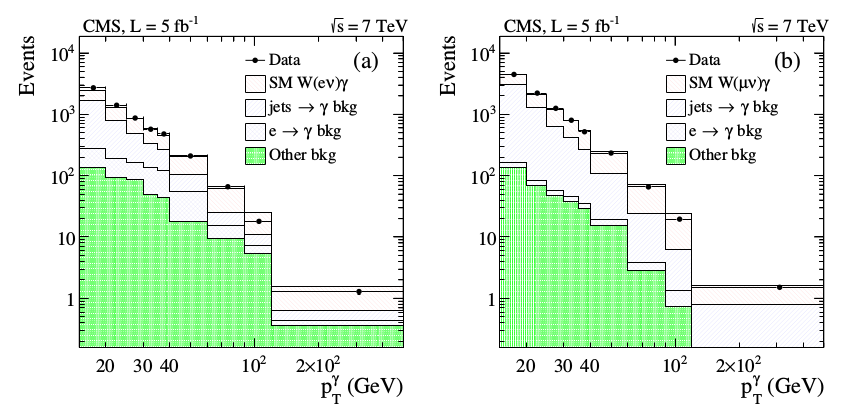
\includegraphics[width=0.80\textwidth]{../figs/WgAbout/Wg7TeV_CMS_ptGamma.png}}
    \caption{The distribution fo the $p_T^\gamma$ of W$\gamma$ candidates in the analysis of 7 TeV CMS data. Data vs signal MC + background estimates. Left: $W\gamma\rightarrow e\nu\gamma$, right: $W\gamma\rightarrow \mu\nu\gamma$. Figure from [REFERENCE]}
    \label{fig:Wg7TeV_CMS_ptGamma}
  \end{center}
\end{figure}


%Background Estimation\\

Events selected according with the criteria described represent a mixture of the signal and background events. The major source of the background is the fake photon background where hadronic jets are misidentified as photons. Such events originate from $W+$jets process mostly but $Z+$jets and $\bar{t}t+$jets events contribute to this source of the background as well. The template method was used as a major method to estimate this background. The shower-shape variable $\sigma_{i\eta i\eta}^{\gamma}$ was used as a discrimination variable. The ratio method was used as a cross check by measuring and comparing the probabilities for jets to pass photon or jets selection criteria. \\

The second major background for the electron channel is the fake photon background where electron can be misidentified as a photon. Such events are coming from $Z+$jets events. Diboson processes contribute to this background for both channels. The fake rates are estimated from the $Z\rightarrow ee$ sample, by checking how often one of the electrons would pass photon selection criteria given the other one passed stringent electron selection criteria.\\

Other sources of backgrounds include real-$\gamma$ backgrounds, fake lepton + real photon and fake lepton + fake photon sources.\\ 

The $p_T^\gamma$ spectra of the selected events in data superimposed with selected events in the simulation of the signal and estimated background contribution for the muon and electron channels are shown in Fig. \ref{fig:Wg7TeV_CMS_ptGamma}. The figure shown a good agreement within the estimated uncertainties.\\

The estimated cross sections are:\\
$\sigma(pp\rightarrow W\gamma \rightarrow e\nu\gamma)$=36.6$\pm$1.2(stat.)$\pm$4.3(syst.)$\pm$0.8(lumi) pb\\
$\sigma(pp\rightarrow W\gamma \rightarrow \mu\nu\gamma)$=37.5$\pm$0.9(stat.)$\pm$4.4(syst.)$\pm$0.8(lumi) pb\\
And the combination result:\\
$\sigma(pp\rightarrow W\gamma \rightarrow l\nu\gamma)$=37.0$\pm$0.8(stat.)$\pm$4.0(syst.)$\pm$0.8(lumi) pb\\

The paper also provides the cross section measurements for $p_T^\gamma>$60 GeV and for $p_T^\gamma>$90 GeV. The combination of two channels for $p_T^\gamma>$60 GeV is $\sigma=$0.76$\pm$0.05(stat.)$\pm$0.08(syst.)$\pm$0.02(lumi) pb while the theoretical NLO prediction is $\sigma=$0.58$\pm$0.08 pb. The result for $p_T^\gamma>$60 GeV is $\sigma=$0.200$\pm$0.025(stat.)$\pm$0.038(syst.)$\pm$0.004(lumi) pb while the theoretical NLO prediction is $\sigma=$0.173$\pm$0.026 pb.\\


\subsubsection{Measurement of the W$\gamma$ cross section in pp collisions at $\sqrt{s}=7$ TeV at ATLAS}
%Wg 7 TeV at ATLAS (2011 and mention 2010)

%Selection

ATLAS collaboration also required each candidate event to have an exactly one lepton, at least one isolated photon and a significant missing transverse energy. The phase space requirements are the same as those for CMS: $p_T^{\gamma}>$ 15 GeV and $\Delta R(l,\gamma)>$0.7 however other selection critea are slightly different: $p_T^l>$ 25 GeV, $E_T^{miss}>$35 GeV, $M_T^W>40$ GeV. In the electron channel Z mass window cut was applied to reduce the contribution from $Z\rightarrow e^+e^-$ events.\\

The sideband method was used to estimate the major background (jets$\rightarrow\gamma$). 

\begin{figure}[htb]
  \begin{center}
    {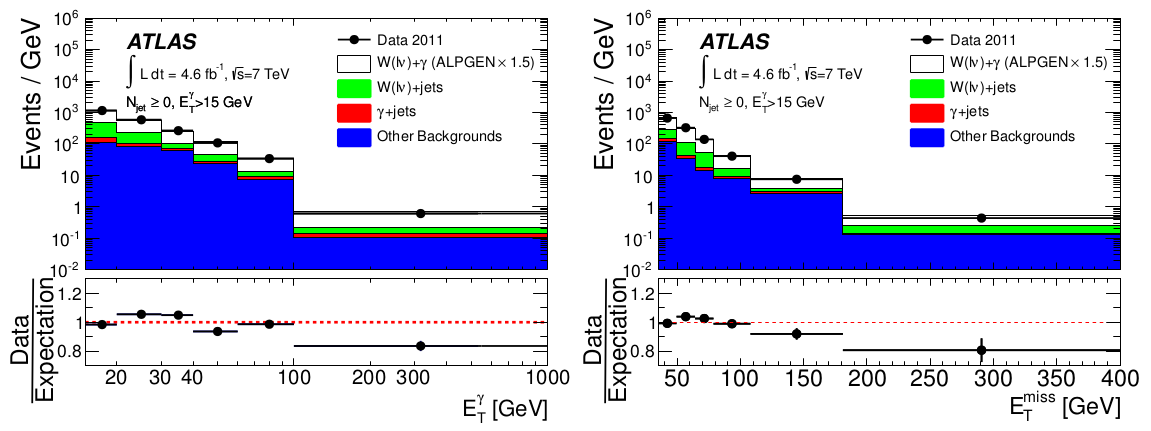
\includegraphics[width=0.80\textwidth]{../figs/WgAbout/Wg7TeV_ATLAS_ptGamma.png}}
    \caption{The distribution fo the $p_T^\gamma$ (left) and $E_T^\gamma$ (right) of W$\gamma$ candidates in the analysis of 7 TeV ATLAS data. Data vs signal MC + background estimates. Figure from [REFERENCE]}
    \label{fig:Wg7TeV_ATLAS_ptGamma}
  \end{center}
\end{figure}


%Background Estimation
%AccXEff
%Pt Spectrum
%Differential and Total CS

%Wg 8 TeV at ATLAS (?)
%NO. DOES NOT EXIST
